\section{Case}
\subsection{Description}

\paragraph{}
The main case of project is based on the analysis of a flow in a turbofan. A turbofan consists in its initial stage of a fan where air entries a high velocity. This fan is a larger compressor than others and split the flow in two, main flow and secondary flow. The secondary flow advances through a conduit but the main flow enters the engine core where it goes throught the compressor stage which is divided in two substages, one of low compression and one of high pressure compressor, where pressure increases. After compression stage, flow enters inside combustion chamber where it is mixed with the fuel and it is burned. Gases obtained pass through the turbines and and arrive at the nozzle, where the air is accelerated and the thrust is obtained.

\begin{figure}[h!]
\centering
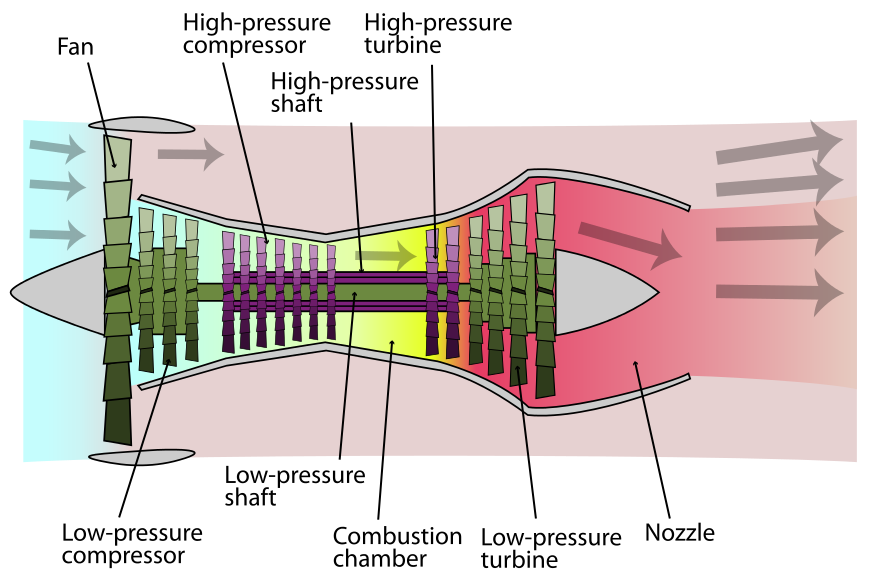
\includegraphics[scale=0.45]{./img/TurbofanEtapas.png}
\caption{First mesh. Toooooo coarse}
\end{figure}

\paragraph{}
The study is centered in the behaviour of the flow in the stage of compression, considering a hypotheses and an initial conditions that will be explained below.

\paragraph{}
The different files of engine to can realise the study, the nacelle,the fan, the combustion chamber, the different stages of compressor and turbine and the nozzle, have been downloaded from the website GrabCad, specifically the files of a \textit{"High Bypass Turbofan Jet Engine"}.

\begin{figure}[h!]
\centering
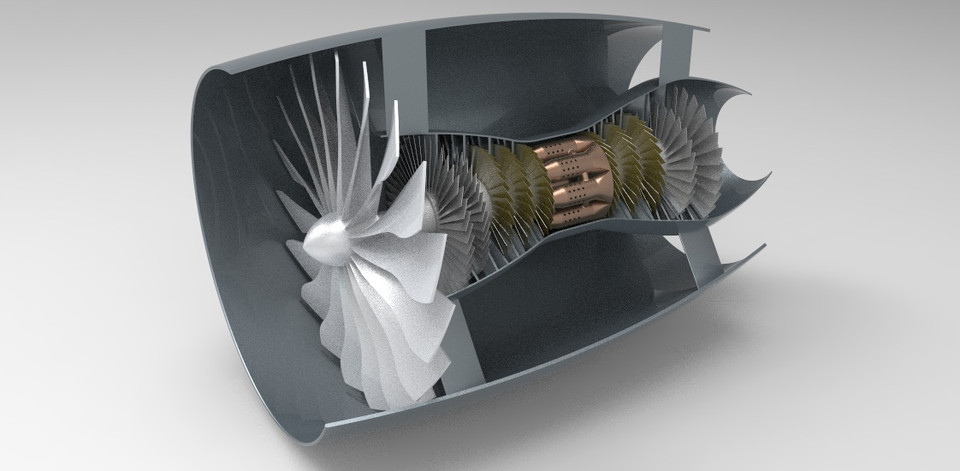
\includegraphics[scale=0.5]{./img/Turbofan.png}
\caption{First mesh. Toooooo coarse}
\end{figure}

\subsection{Hypotheses}

\begin{itemize}

	\item Tridimensional flow
	\item Viscous flow
	\item Compressible flow
	\item Newtonian flow
	\item Stationary flow

\end{itemize}




